\documentclass{tum_report}
\usepackage{amsmath}
\usepackage{amssymb}
\usepackage{float}
\usepackage{graphicx}
\usepackage{enumitem}
\usepackage{verbatim}
\usepackage{booktabs}
\usepackage{array}
\usepackage{xcolor}
\usepackage{hyperref}

\begin{document}
    \ministry{MINISTRY OF EDUCATION, CULTURE AND RESEARCH\\OF THE REPUBLIC OF MOLDOVA}


\university{\textbf{Technical University of Moldova}}
\faculty{\textbf{Faculty of Computers, Informatics and Microelectronics}}
\department{\textbf{Department of Software Engineering and Automatics}}

\title{Computer Graphics}

\year{2026}

\begin{titlepage}
    \centering

    % --- Logo ---
    
\includegraphics[width=0.25\textwidth]{./UTM_Logo.png}\par\vspace{1cm}

    % --- Ministry and University info ---
    {\bfseries
        \textsc{\ministryname} \\[0.15cm]
        \universityname\\[-0.01cm]
        \facultyname\\[-0.01cm]
        \departmentname
    }\par


    \vspace{2.5cm}

    % --- Student info ---
    \textbf{Mihail Pancenco} \textbf{FAF-243}\par

    \vspace{-0.5cm}

    % --- Title section ---
    {\Large \textbf{Report}\par} \normalsize	
    \vspace{0.5cm}
    {\normalfont\Large \textit{Laboratory work n. 3}\par}
    \vspace{-0.5cm}
    \Large \textit{of Operating Systems}\par \normalsize	

    \huge \textit{The Command Line: Shell, Pipes and Text Filters}\par \normalsize	
    

    \vspace{3cm}

    % --- Checked by section ---
    \begin{flushright}
        {\normalfont
            Supervisers:\par
            \textbf{Dumitrașcu Marius}, \textit{University assistant}\par
            \textbf{Reițman Patricia}, \textit{University assistant}\par
            DISA, FCIM, UTM
        }
    \end{flushright}
    
    

    \vfill{}

    % --- Footer ---
    \textbf{Chișinău -- \degreeyear}\par

\end{titlepage}


    \clearpage
    \addtocontents{toc}{\protect\thispagestyle{empty}}
    \tableofcontents
    \thispagestyle{empty}
    \clearpage

% =======================================================================
\chapter{Introduction}
% =======================================================================

The command line provides direct access to the operating system through a
shell. Bash can interpret commands, expand filenames and variables, connect
programs through pipes, redirect input and output, and automate repeated
operations. These facilities are particularly useful when working with
files, processes, and structured text.

The work focuses on navigating Bash efficiently, examining how it interprets
command lines, and combining standard Unix utilities to answer questions
about a web access log. It also covers writing a small shell script and
scheduling its execution.

\clearpage
% =======================================================================
\chapter{Before we start}
% =======================================================================

The commands are executed in Bash on an Ubuntu virtual machine. A working
directory is created at \texttt{\textasciitilde/os-lab3}, together with an
artificial web access log used for the text-processing exercises.

Each log entry contains a date, time, username, request status, and page.
A Bash loop generates 500 entries; the status alternates according to the
loop counter, while usernames and pages repeat in fixed cycles. The first
three lines and the line count are displayed to check the generated data.

\begin{figure}[H]
    \centering
    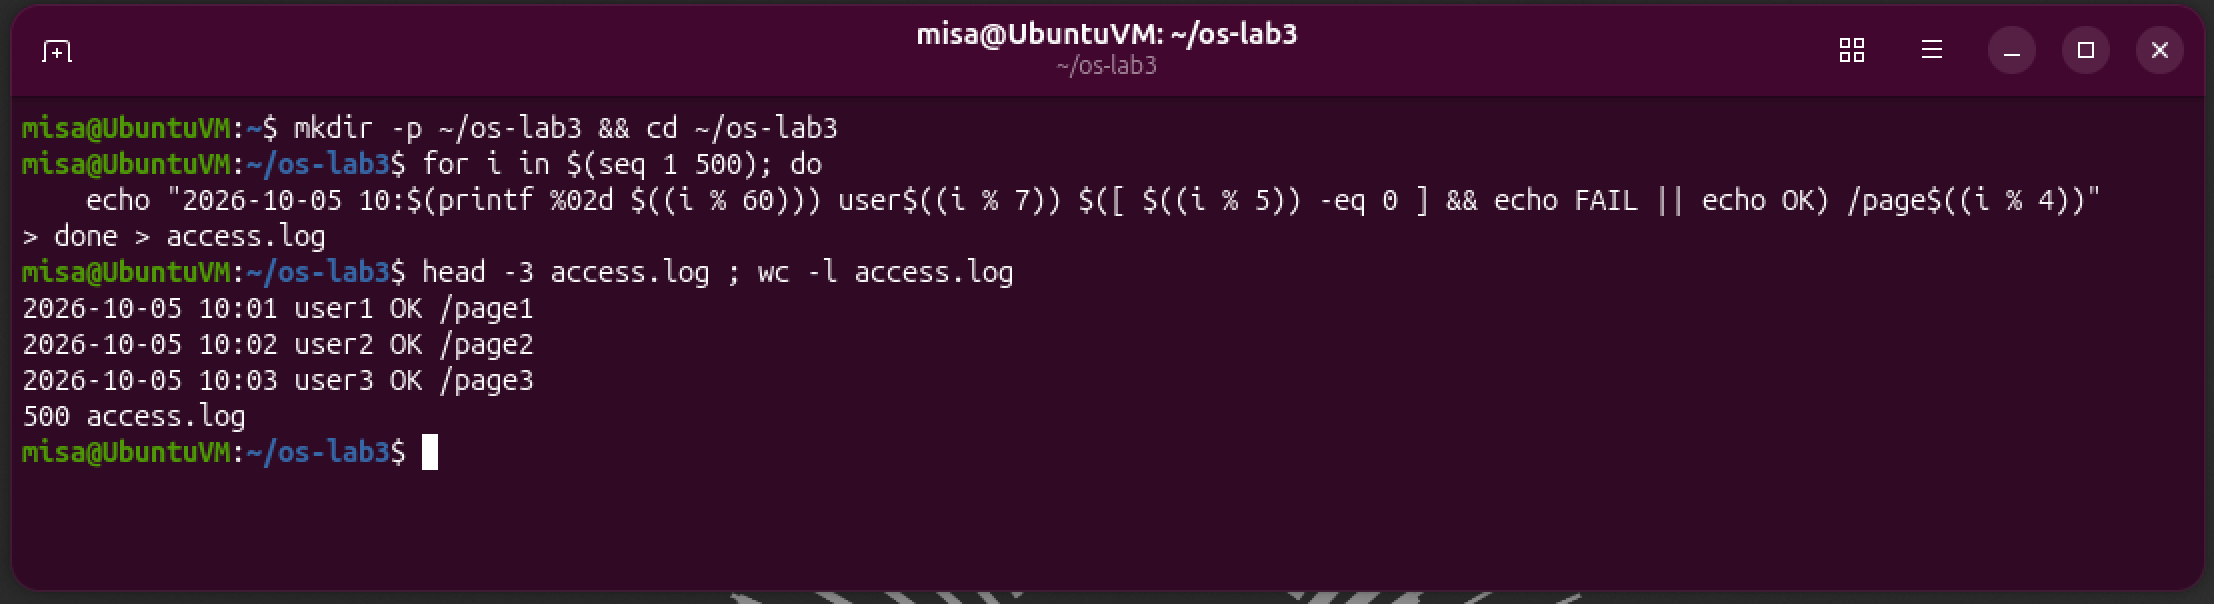
\includegraphics[width=0.88\textwidth,height=0.76\textheight,keepaspectratio]{./img/img_01.png}
    \caption{Generating the access log and verifying its 500 entries}
    \label{fig:log_generation}
\end{figure}

The resulting \texttt{access.log} contains 500 requests and is ready for
further analysis.

% =======================================================================
\chapter{Tasks}
% =======================================================================

\section{Move fast, find help}

Bash provides filename and directory completion using the Tab key. Entering
an incomplete path under \texttt{/usr/sh} and pressing Tab completes it to
\texttt{/usr/share/}. Likewise, entering \texttt{cd /et} and pressing Tab
completes the path to \texttt{/etc/}. Completion reduces repetitive typing
and helps locate existing paths.

The command history can be searched without repeatedly using the arrow keys.
After running \texttt{echo}, \texttt{ls}, and \texttt{wc}, pressing
\texttt{Ctrl+R} and entering \texttt{ec} locates the earlier
\texttt{echo something} command. Pressing Enter executes that command again.

\begin{figure}[H]
    \centering
    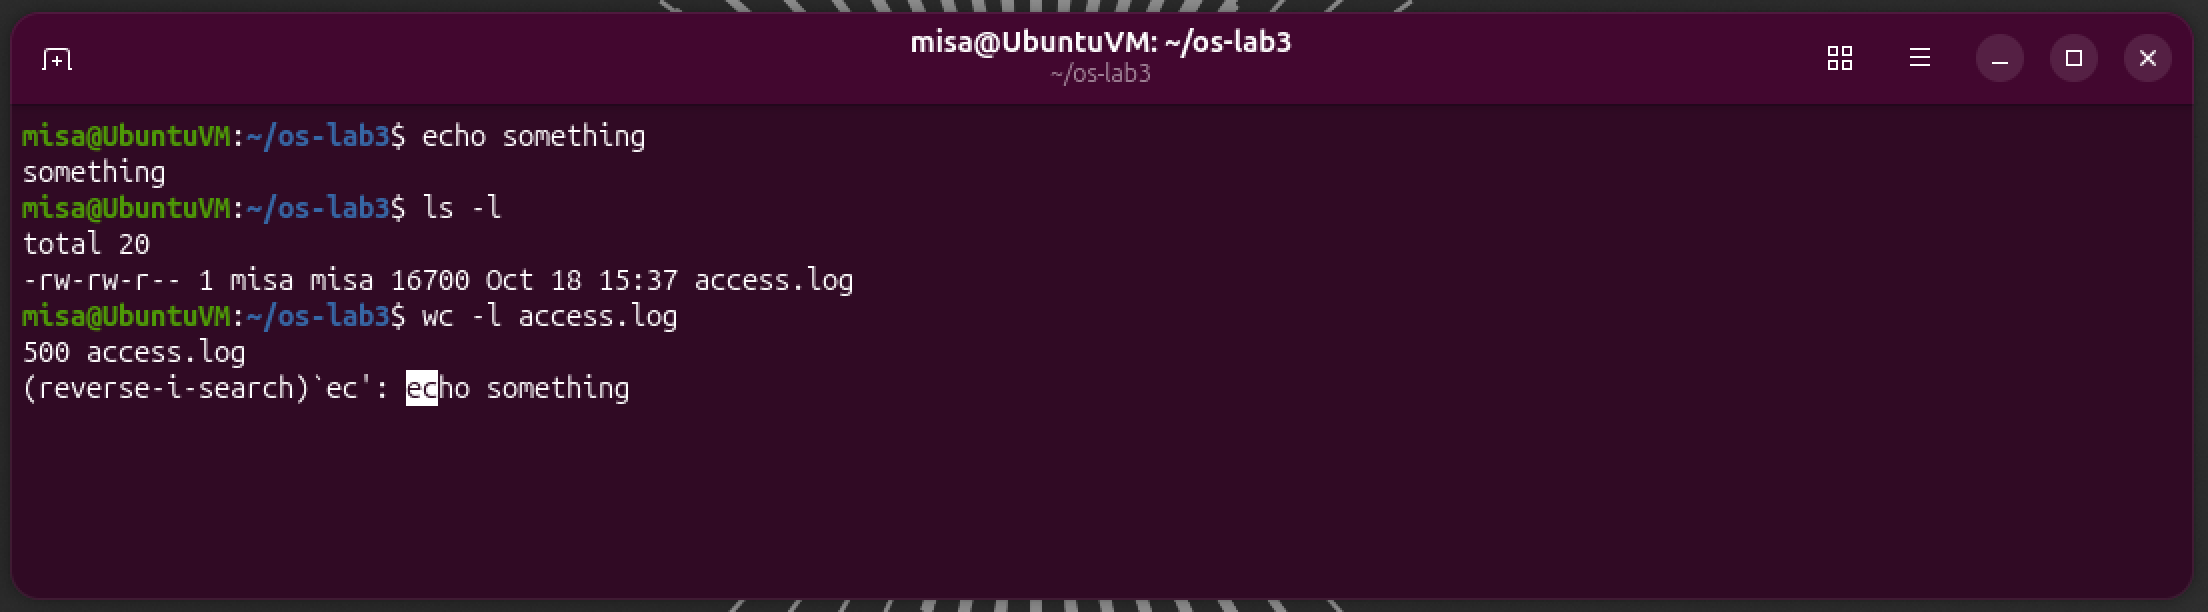
\includegraphics[width=0.88\textwidth,height=0.76\textheight,keepaspectratio]{./img/img_02.png}
    \caption{Command history and reverse incremental search}
    \label{fig:reverse_history}
\end{figure}

Commands may be implemented inside Bash or provided by separate executables.
The \texttt{type} command identifies \texttt{cd} and \texttt{echo} as shell
built-ins. In the current environment, \texttt{ls} is an alias for
\texttt{ls --color=auto}, and the executable is located at
\texttt{/usr/bin/ls}. The shell searches directories named in its
\texttt{PATH} variable to find external commands. The current \texttt{PATH}
contains ten entries, including a repeated \texttt{/snap/bin} entry.

The \texttt{tr} utility is used to replace the colon separators in
\texttt{PATH} with newline characters, making each directory visible on its
own line. An attempt to run \texttt{nosuchprog} fails with exit status 127.
The variable \texttt{\$?} holds the exit status of the most recently
completed foreground command.

\begin{figure}[H]
    \centering
    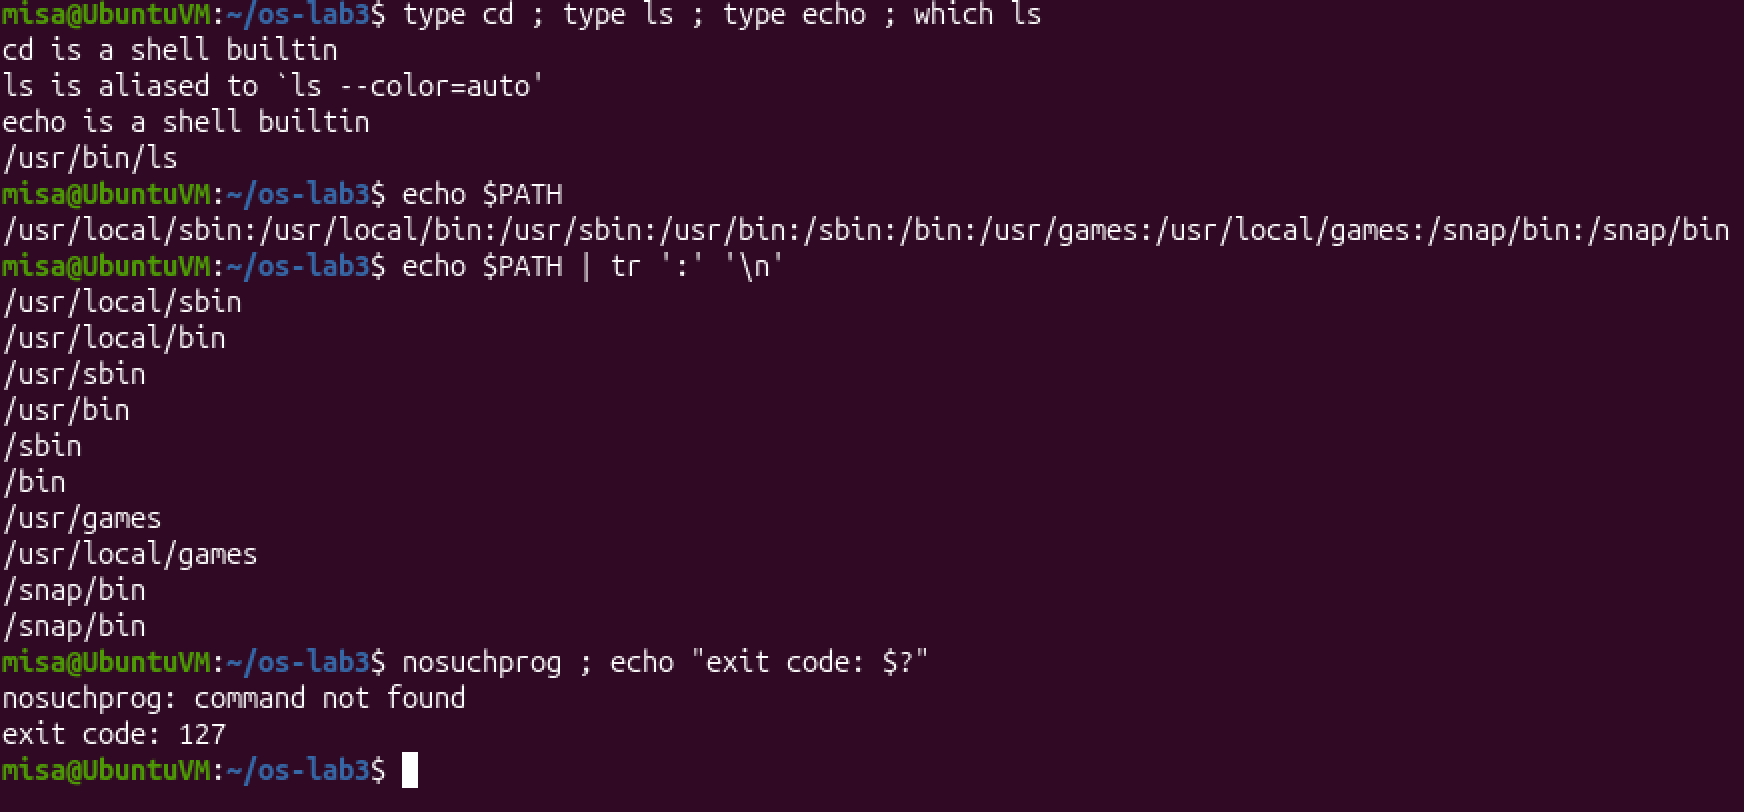
\includegraphics[width=0.88\textwidth,height=0.76\textheight,keepaspectratio]{./img/img_03.png}
    \caption{Built-in commands, executable lookup, PATH and exit status}
    \label{fig:command_lookup}
\end{figure}

Manual pages are available directly in the terminal. In \texttt{man ls},
searching for \texttt{sort} reveals the \texttt{-t} option and the
\texttt{--sort=time} form, which order entries by modification time.
The \texttt{n} key moves to the next match, and \texttt{q} closes the manual.

\begin{figure}[H]
    \centering
    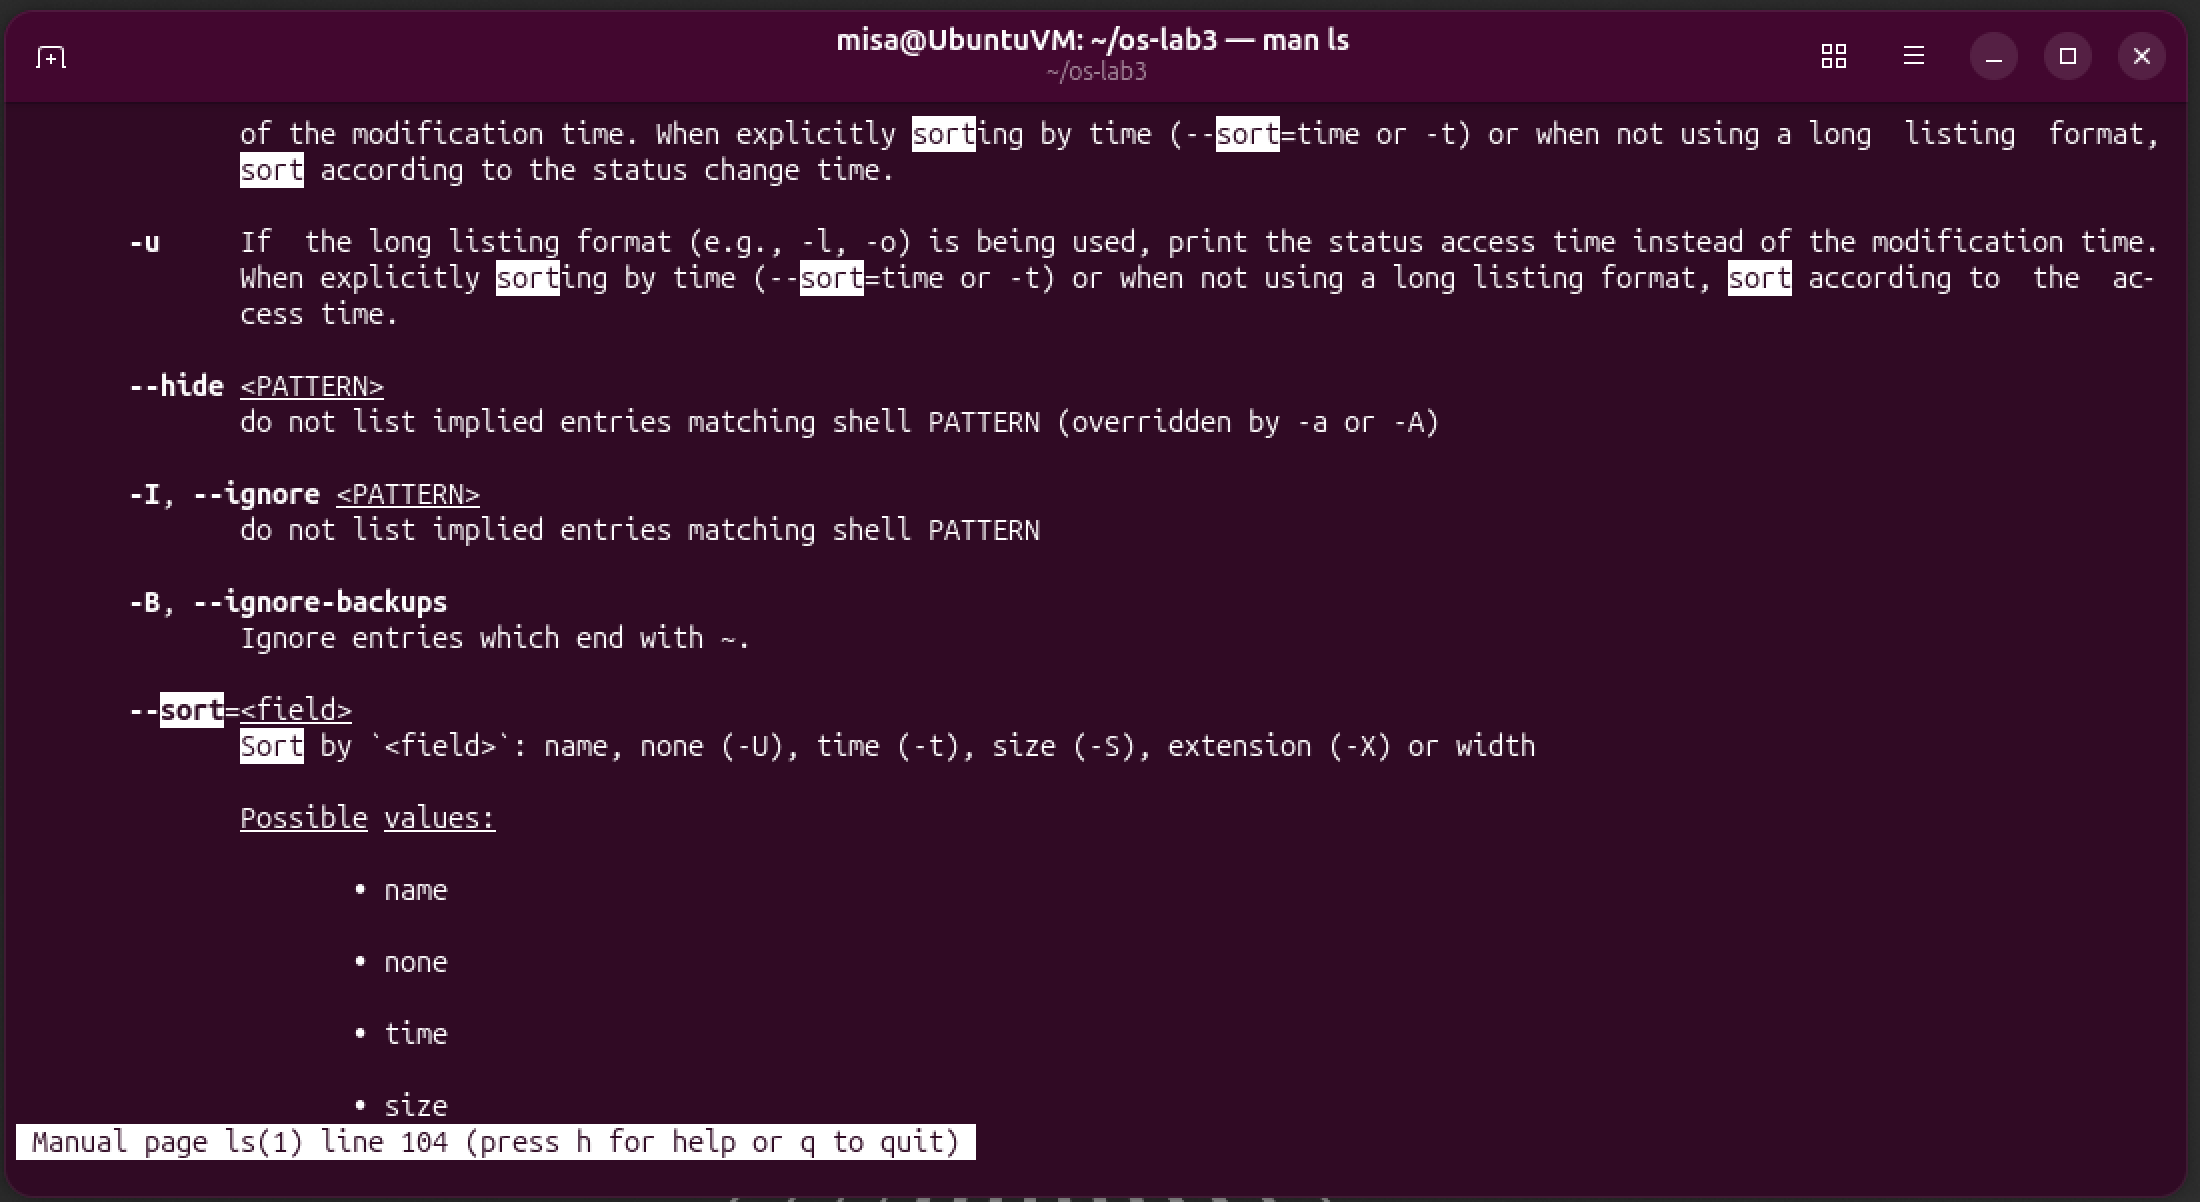
\includegraphics[width=0.88\textwidth,height=0.76\textheight,keepaspectratio]{./img/img_04.png}
    \caption{Finding the sorting option in the ls manual page}
    \label{fig:man_ls}
\end{figure}

Additional help is available through \texttt{ls --help},
\texttt{man -k}, and the shell's \texttt{help} command. The first displays
option documentation, \texttt{man -k} searches manual descriptions by
keyword, and \texttt{help cd} describes Bash's built-in directory command.

\begin{figure}[H]
    \centering
    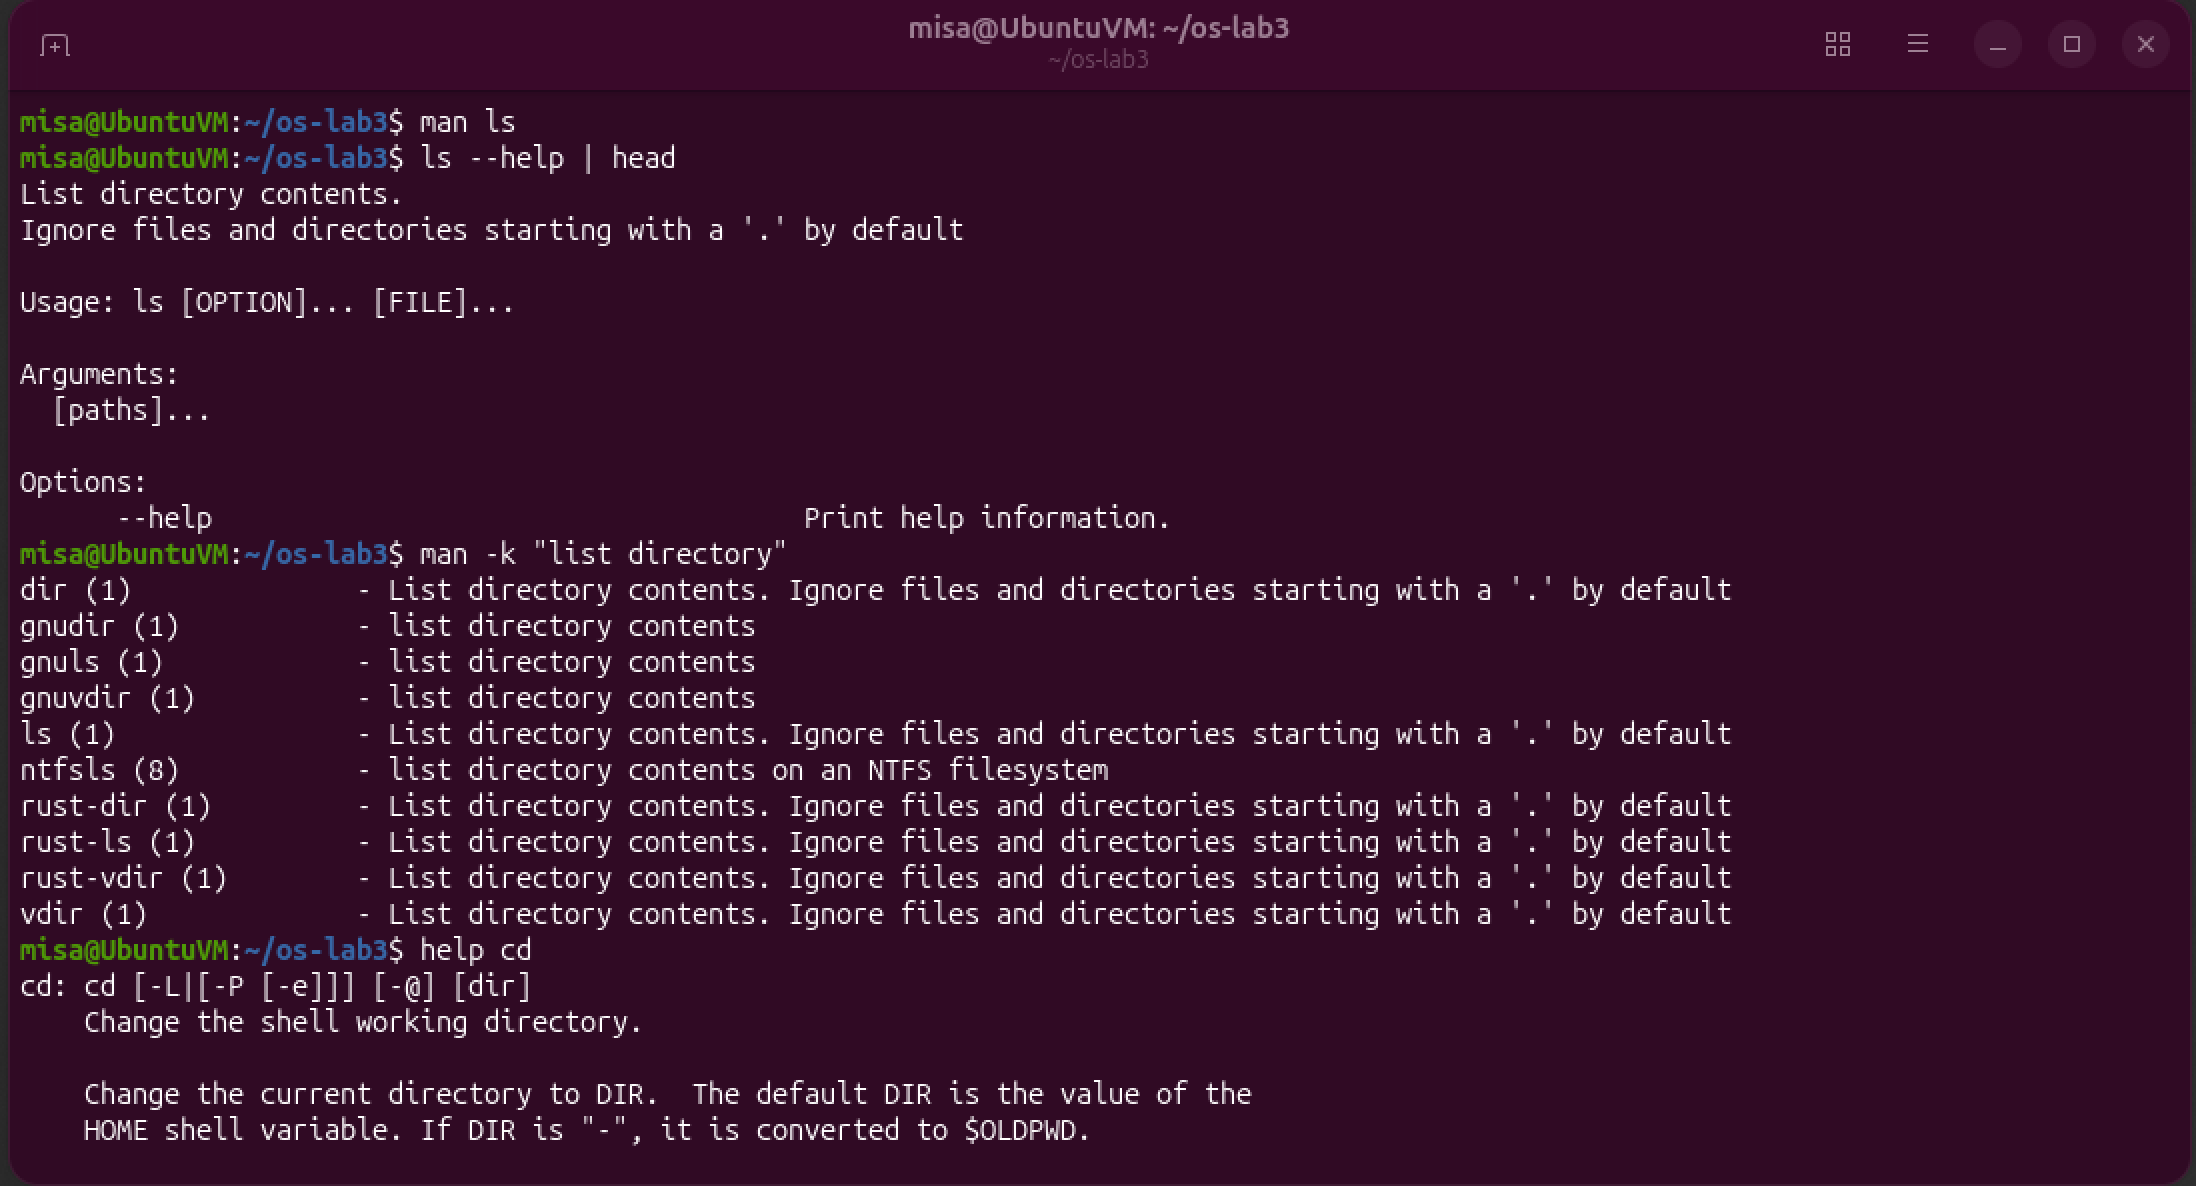
\includegraphics[width=0.88\textwidth,height=0.76\textheight,keepaspectratio]{./img/img_05.png}
    \caption{Command help, manual keyword search and built-in help}
    \label{fig:shell_help}
\end{figure}

\begin{figure}[H]
    \centering
    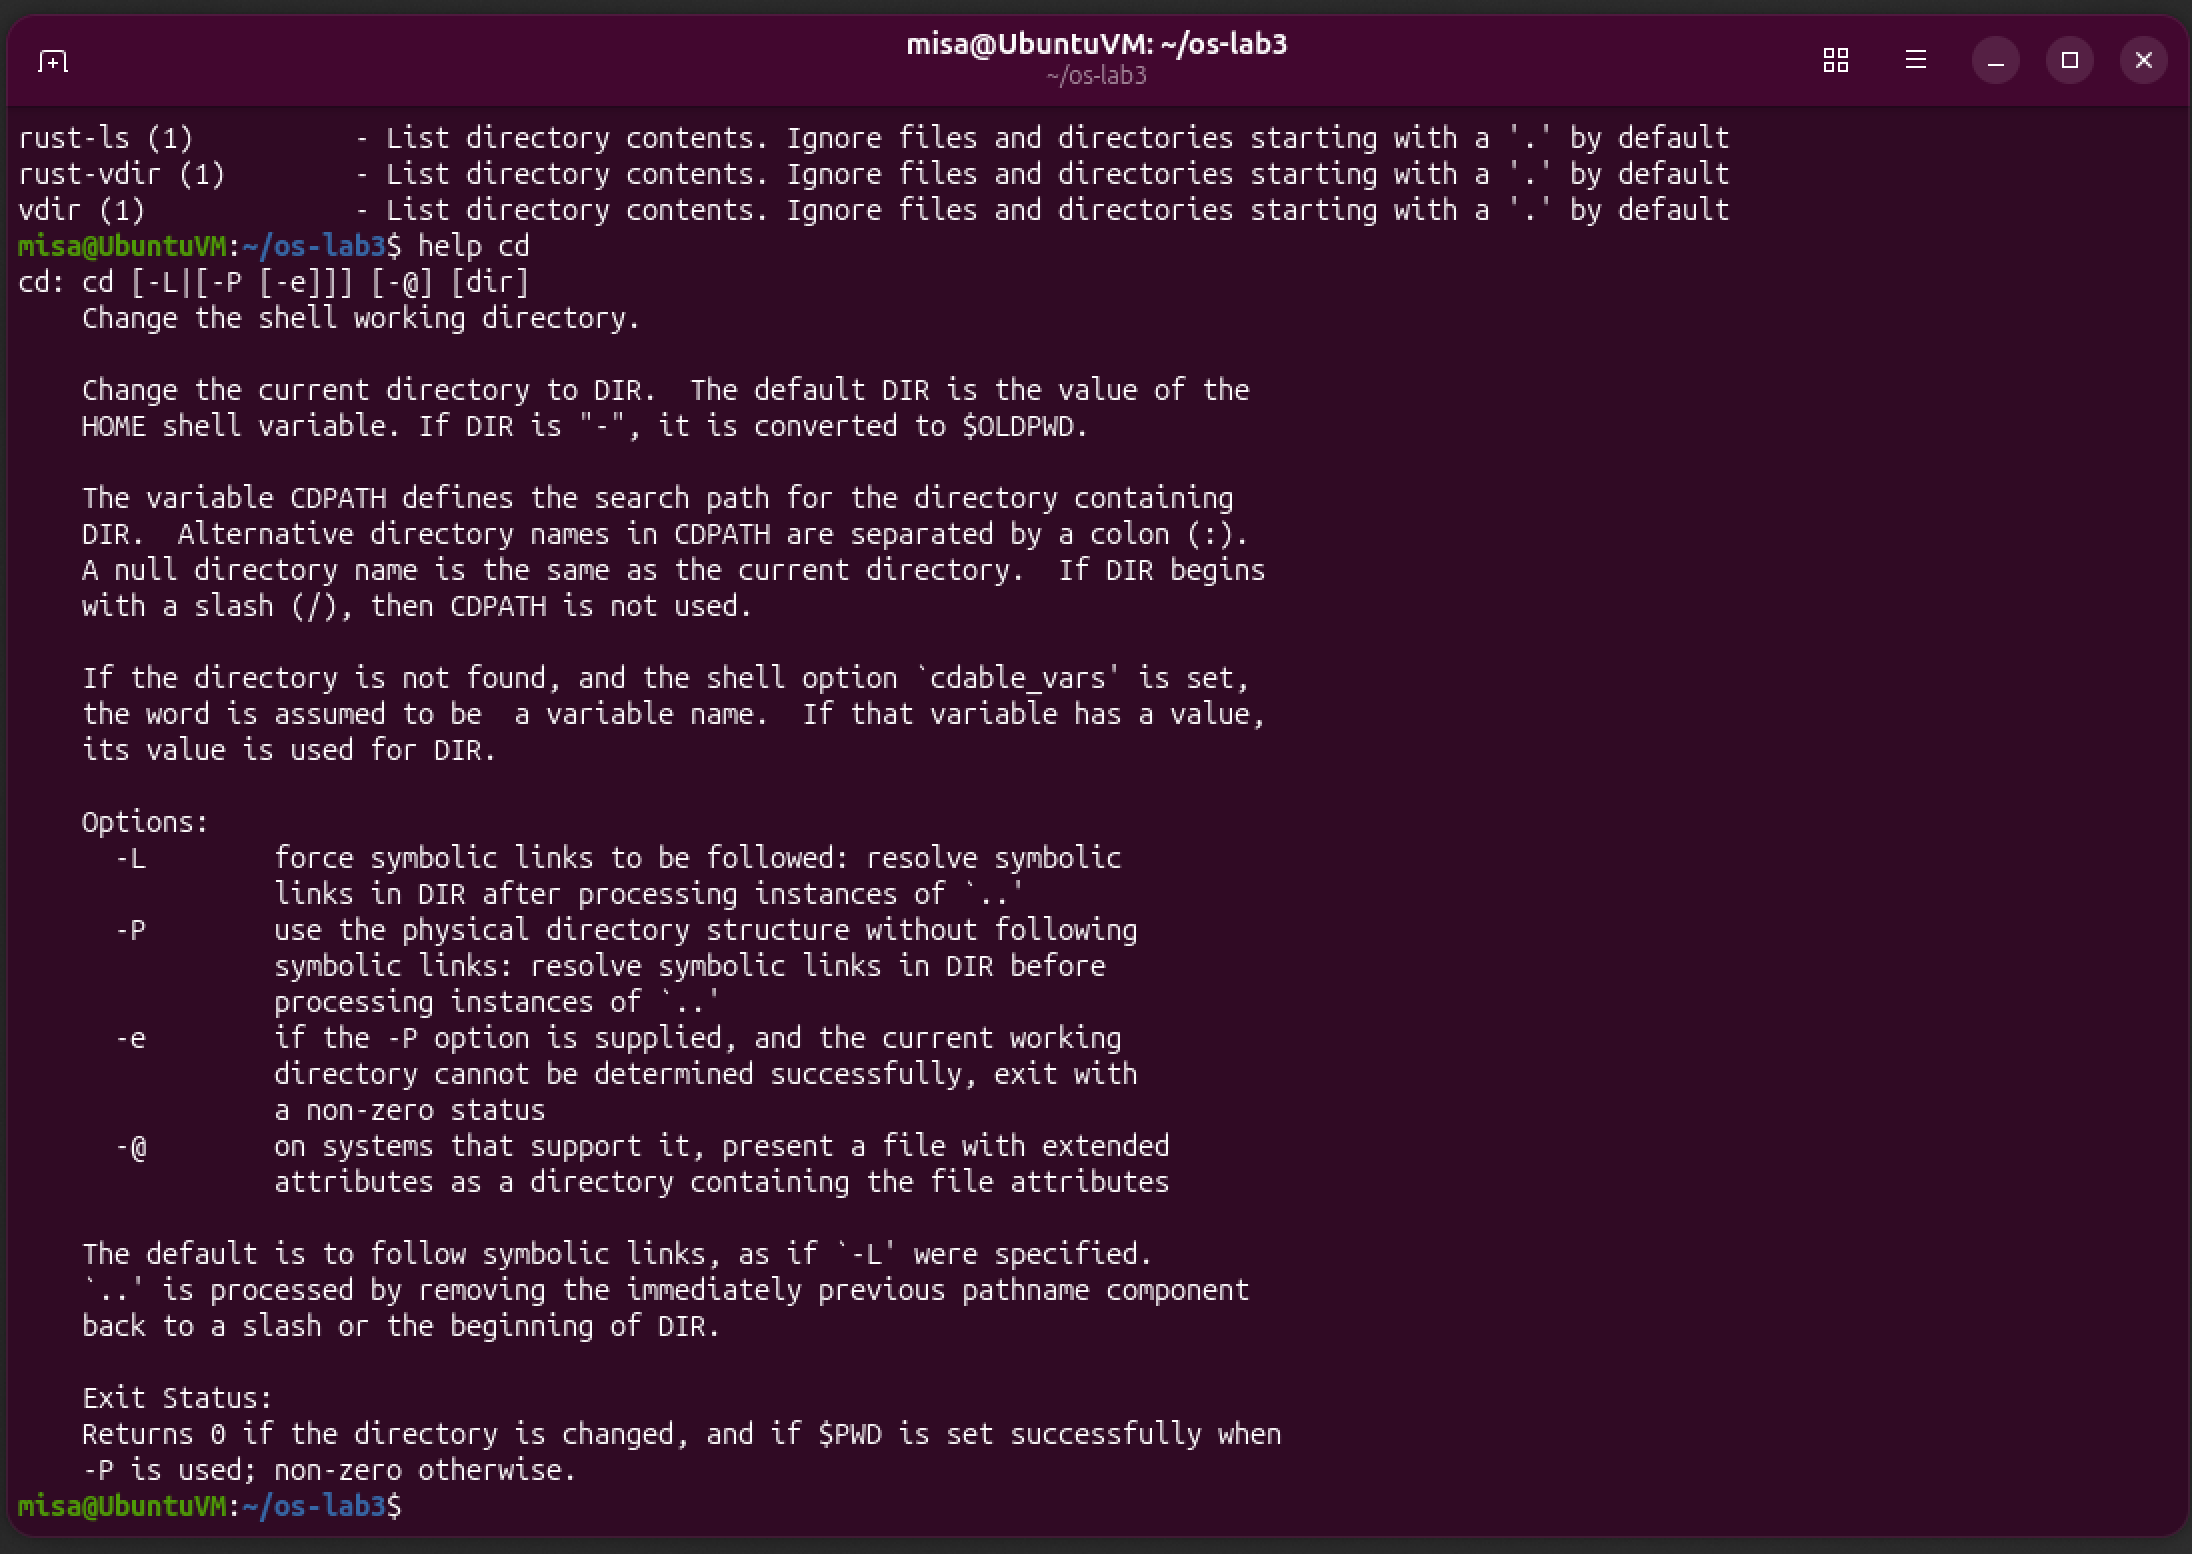
\includegraphics[width=0.88\textwidth,height=0.76\textheight,keepaspectratio]{./img/img_06.png}
    \caption{Additional documentation for the cd shell built-in}
    \label{fig:help_cd}
\end{figure}

\subsection{Observations}
\begin{enumerate}
    \item \textbf{Which of cd, ls and echo are built-ins, and why must cd be one?}
    \texttt{cd} and \texttt{echo} are Bash built-ins; \texttt{ls} resolves
    to an alias that invokes an external executable. Changing a directory
    must affect the current shell process. A separate program would change
    only its own working directory.

    \item \textbf{How many directories are in PATH, and where is ls?}
    There are ten \texttt{PATH} entries, with nine distinct directories.
    The \texttt{ls} executable is at \texttt{/usr/bin/ls}.

    \item \textbf{What exit code does a missing command return?}
    Bash returned 127 for \texttt{nosuchprog}.

    \item \textbf{Which ls option sorts by modification time?}
    The option is \texttt{-t}, also available as \texttt{--sort=time}.
\end{enumerate}

\section{What the shell does to your line}

A separate \texttt{play} directory is populated with C source filenames,
text filenames, and a filename containing a space. The shell processes
expansions and quoting before it invokes a command. This is visible even
with \texttt{echo}, which simply prints the arguments it receives.

The patterns \texttt{*.c}, \texttt{file?.txt}, and \texttt{[a-b]*} are
expanded by Bash to matching filenames. The asterisk matches any sequence
of characters; a question mark matches one character; and a bracket
expression matches one character from a specified set or range. When no
filename matches \texttt{*.xyz}, Bash leaves that pattern unchanged under
its default settings.

A filename containing spaces must be passed as one argument. The unquoted
command \texttt{ls alfa beta.txt} searches for two separate names and fails.
Quoting the filename makes the command work. Bash also distinguishes single
quotes, double quotes, and backslash escaping: single quotes preserve text,
double quotes permit variable expansion, and a backslash protects the next
character from special interpretation.

Brace expansion generates the numbers 1 through 5 and the filenames
\texttt{log1.txt} to \texttt{log3.txt}. Arithmetic expansion evaluates
\texttt{7 * 6} to 42. Command substitution inserts the output of
\texttt{date} and \texttt{whoami} into a larger string; the date format
\texttt{\%A} requests the full weekday name.

\begin{figure}[H]
    \centering
    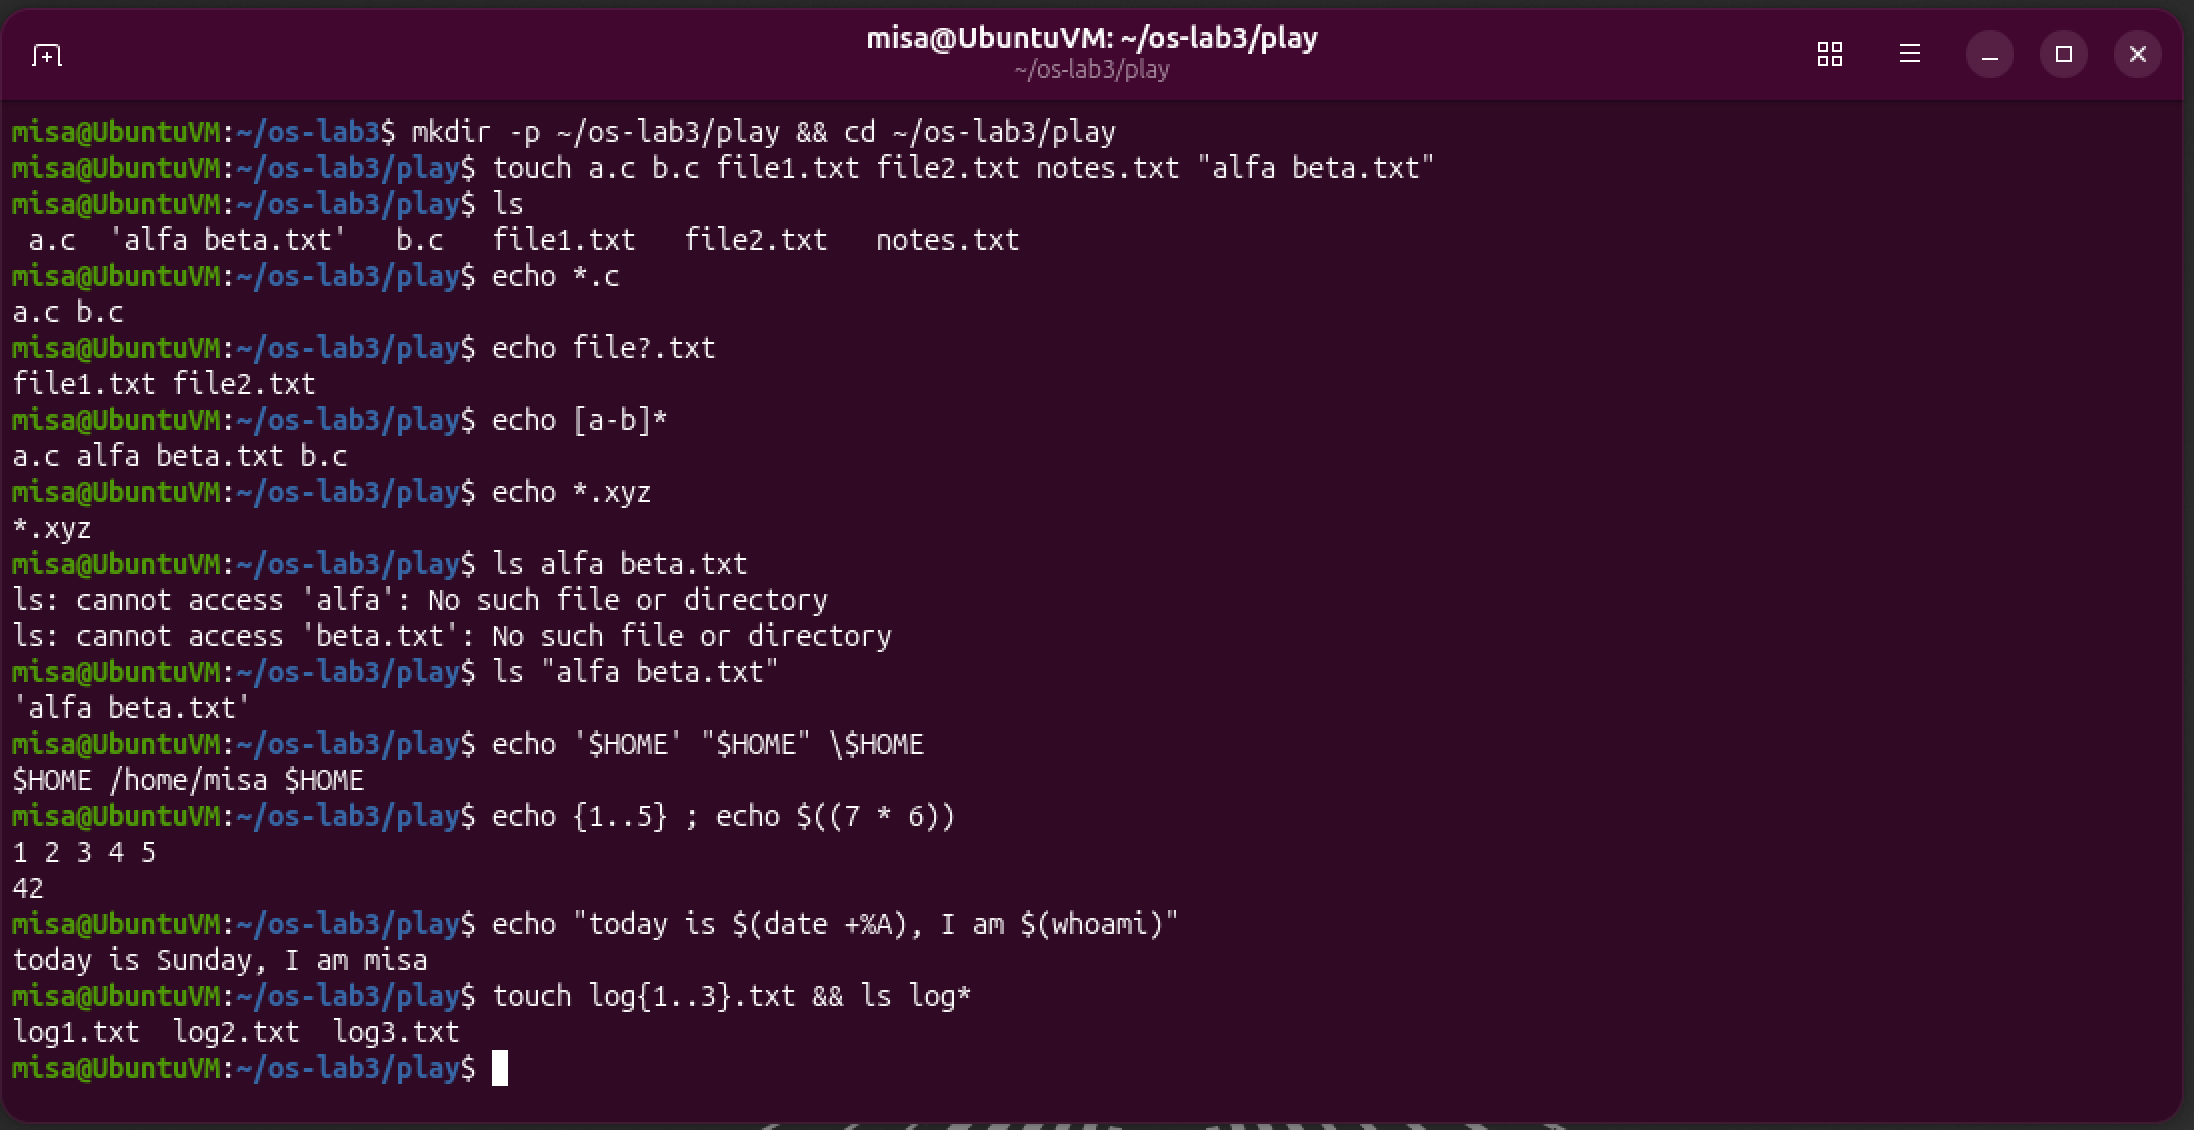
\includegraphics[width=0.88\textwidth,height=0.76\textheight,keepaspectratio]{./img/img_07.png}
    \caption{Filename patterns, quoting and Bash expansions}
    \label{fig:bash_expansions}
\end{figure}

\subsection{Observations}
The predicted and observed outputs agreed for most commands. Three details
required correction: an unmatched \texttt{*.xyz} pattern was printed
literally, the backslash preceding \texttt{\$HOME} disappeared while
preventing expansion, and \texttt{date +\%A} produced the full weekday name.

\begin{enumerate}[leftmargin=*,itemsep=2pt]
    \item \texttt{echo *.c}: predicted and observed \texttt{a.c b.c}.
    \item \texttt{echo file?.txt}: predicted and observed
    \texttt{file1.txt file2.txt}.
    \item \texttt{echo [a-b]*}: predicted and observed the names beginning
    with \texttt{a} or \texttt{b}, including \texttt{alfa beta.txt}.
    \item \texttt{echo *.xyz}: predicted an empty result; observed the literal
    pattern \texttt{*.xyz}, because no file matched it.
    \item \texttt{ls alfa beta.txt}: predicted and observed two
    \texttt{No such file or directory} errors.
    \item \texttt{ls "alfa beta.txt"}: predicted and observed the single
    matching filename. The displayed quotes are formatting added by
    \texttt{ls}.
    \item \texttt{echo} with three forms of \texttt{\$HOME}: predicted
    literal text for single quotes and a path for double quotes;
    observed \texttt{\$HOME /home/misa \$HOME}. The backslash is consumed
    during escaping rather than printed.
    \item Brace and arithmetic expansion: predicted and observed
    \texttt{1 2 3 4 5} followed by \texttt{42}.
    \item Command substitution: expected an inserted day and username,
    without knowing the weekday format; observed
    \texttt{today is Sunday, I am misa}.
    \item The \texttt{touch} command with brace expansion: predicted and
    observed three files named \texttt{log1.txt}, \texttt{log2.txt}, and
    \texttt{log3.txt}.
\end{enumerate}

Bash performs glob expansion before executing \texttt{echo}. The unquoted
filename with a space is split into two arguments; it can be fixed using
\texttt{ls "alfa beta.txt"} or by escaping the space. Single quotes prevent
expansion; double quotes allow variable and command substitution while
preserving spaces inside the argument.

\section{Redirection, chaining and jobs}

Unix processes receive three standard file descriptors: standard input
(0), standard output (1), and standard error (2). Redirection changes
where these streams are read or written. Redirecting output with
\texttt{>} creates or overwrites a file, while \texttt{>>} appends to it.

The command that lists \texttt{/etc} and a nonexistent \texttt{/nope} path
writes the directory listing to \texttt{out.txt} and the error message to
\texttt{err.txt} using \texttt{2>}. The listing contains 238 lines in the
recorded run. Redirecting both streams with \texttt{> all.txt 2>\&1}
places them in the same file: \texttt{2>\&1} makes descriptor 2 point to
the current destination of descriptor 1.

Redirections are applied from left to right. In the reversed form
\texttt{2>\&1 > reverse.txt}, standard error continues to point to the
terminal while standard output goes to the file. The two forms can
therefore produce different output locations even though they contain the
same operators.

\begin{figure}[H]
    \centering
    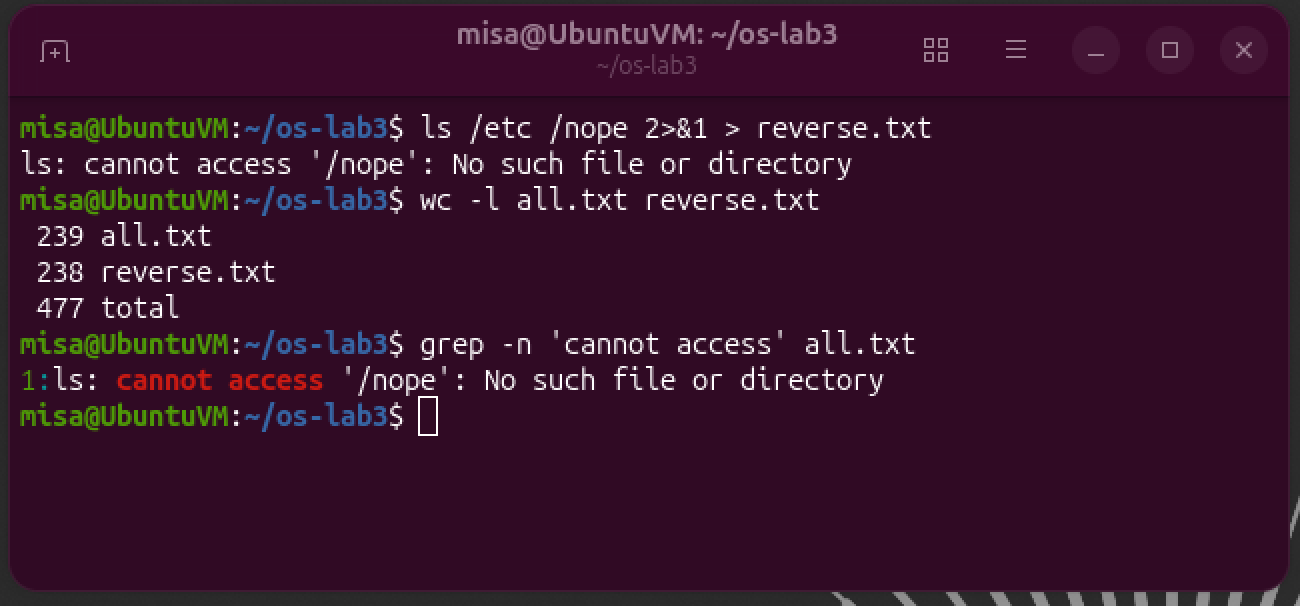
\includegraphics[width=0.88\textwidth,height=0.76\textheight,keepaspectratio]{./img/img_09.png}
    \caption{Comparing the two redirection orders}
    \label{fig:redirection_order}
\end{figure}

Input redirection with \texttt{<} supplies file contents to standard input.
Thus, \texttt{wc -l < access.log} prints \texttt{500} without a filename,
whereas naming the file as an argument also displays \texttt{access.log}.
The special file \texttt{/dev/null} can discard unwanted error output.

The shell also supports conditional execution. A semicolon separates
commands without imposing a success condition. The \texttt{\&\&} operator
runs the next command only if the previous command succeeded; \texttt{||}
runs it only if the previous command failed. The variable \texttt{\$?}
provides the last exit status, which is 2 in the recorded missing-path
example.

Finally, appending \texttt{\&} starts \texttt{sleep 100} as a background
job. The \texttt{jobs} command lists active shell jobs, and
\texttt{kill \%1} sends a termination signal to job 1.

\begin{figure}[H]
    \centering
    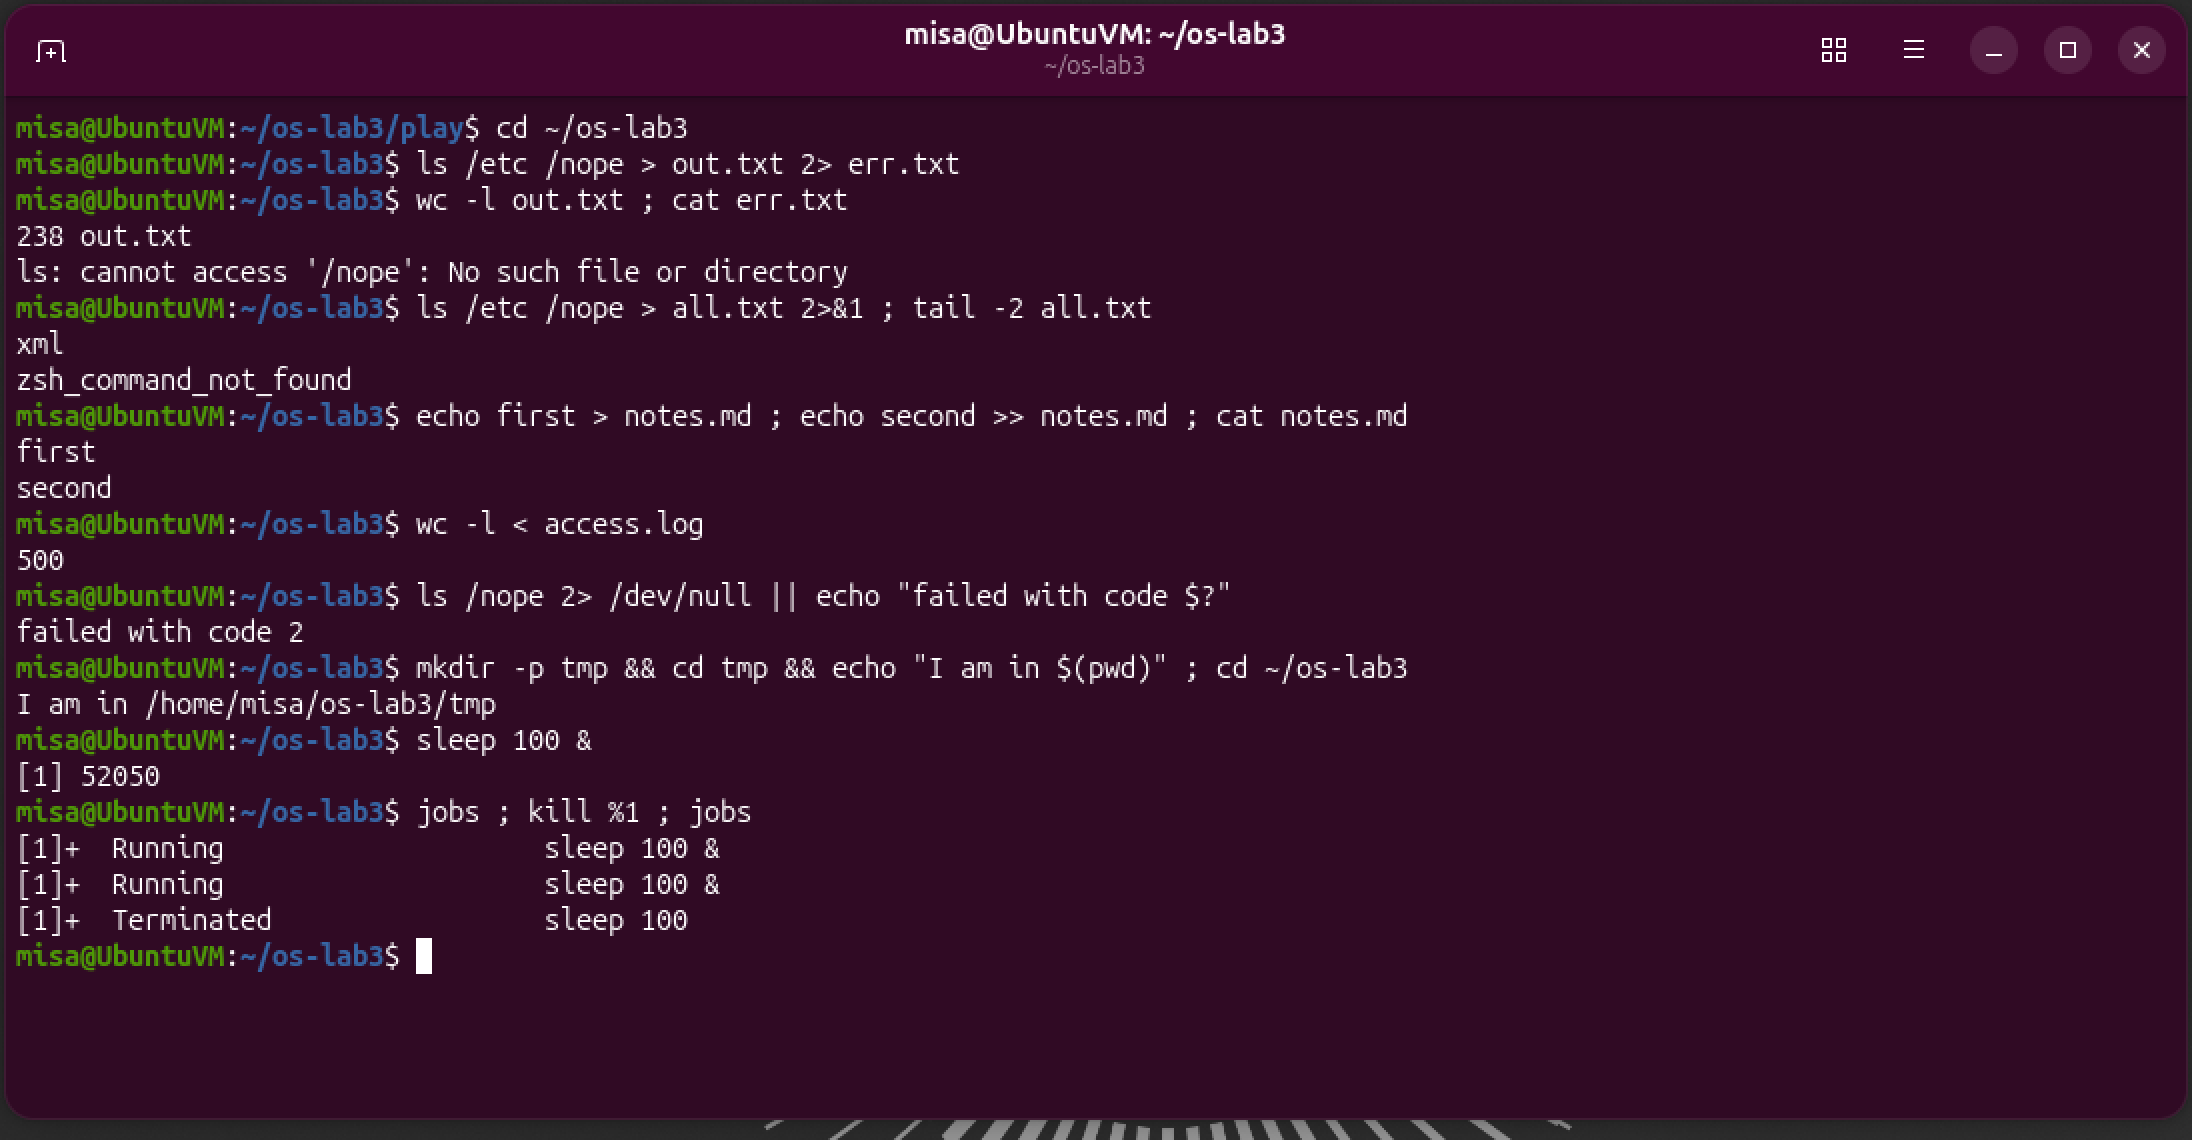
\includegraphics[width=0.88\textwidth,height=0.76\textheight,keepaspectratio]{./img/img_08.png}
    \caption{Output redirection, conditional commands and background jobs}
    \label{fig:redirection_jobs}
\end{figure}

\subsection{Observations}
\begin{enumerate}
    \item \textbf{Which file received the error and which the listing?}
    The directory listing was written to \texttt{out.txt}; the error about
    \texttt{/nope} was written to \texttt{err.txt}.
    \item \textbf{How do the two orders of redirection differ?}
    With \texttt{> all.txt 2>\&1}, both streams go to the file. With
    \texttt{2>\&1 > reverse.txt}, the error remains on the terminal and the
    directory listing goes to \texttt{reverse.txt}; Bash processes the
    redirections left to right.
    \item \textbf{Why does input redirection change the wc output?}
    With \texttt{< access.log}, \texttt{wc} reads unnamed standard input.
    With \texttt{wc -l access.log}, it knows and prints the filename.
    \item \textbf{What do the chaining operators mean?}
    \texttt{;} runs commands in sequence; \texttt{\&\&} requires success
    before continuing; \texttt{||} requires failure before continuing.
\end{enumerate}

\section{Answer questions with one-liners}

The access log is analysed through pipelines of small text-processing
utilities. \texttt{grep} selects matching records, \texttt{cut} extracts
fields, \texttt{sort} orders values, \texttt{uniq -c} counts adjacent equal
values, and \texttt{wc -l} counts lines. Every question is represented by
one executable command line in \texttt{oneliners.sh}.

The 500 requests contain 100 failures. Four distinct pages occur:
\texttt{/page0}, \texttt{/page1}, \texttt{/page2}, and \texttt{/page3},
each requested 125 times. The highest number of failed requests is shared
by \texttt{user3} and \texttt{user5}, with 15 each. In total,
\texttt{user3} made 72 requests, of which 15 failed. The last three failed
requests are \texttt{10:10 user0}, \texttt{10:15 user5}, and
\texttt{10:20 user3}.

The remaining two questions concern the local operating system.
The seventh field of \texttt{/etc/passwd} records the configured account
shell; counting its distinct values reveals how many accounts use each
shell on the current machine. The results depend on the machine's installed
accounts. Finally, \texttt{ls -l /etc | wc -l} counts one additional line
because the long listing begins with a \texttt{total} header.

\begin{figure}[H]
    \centering
    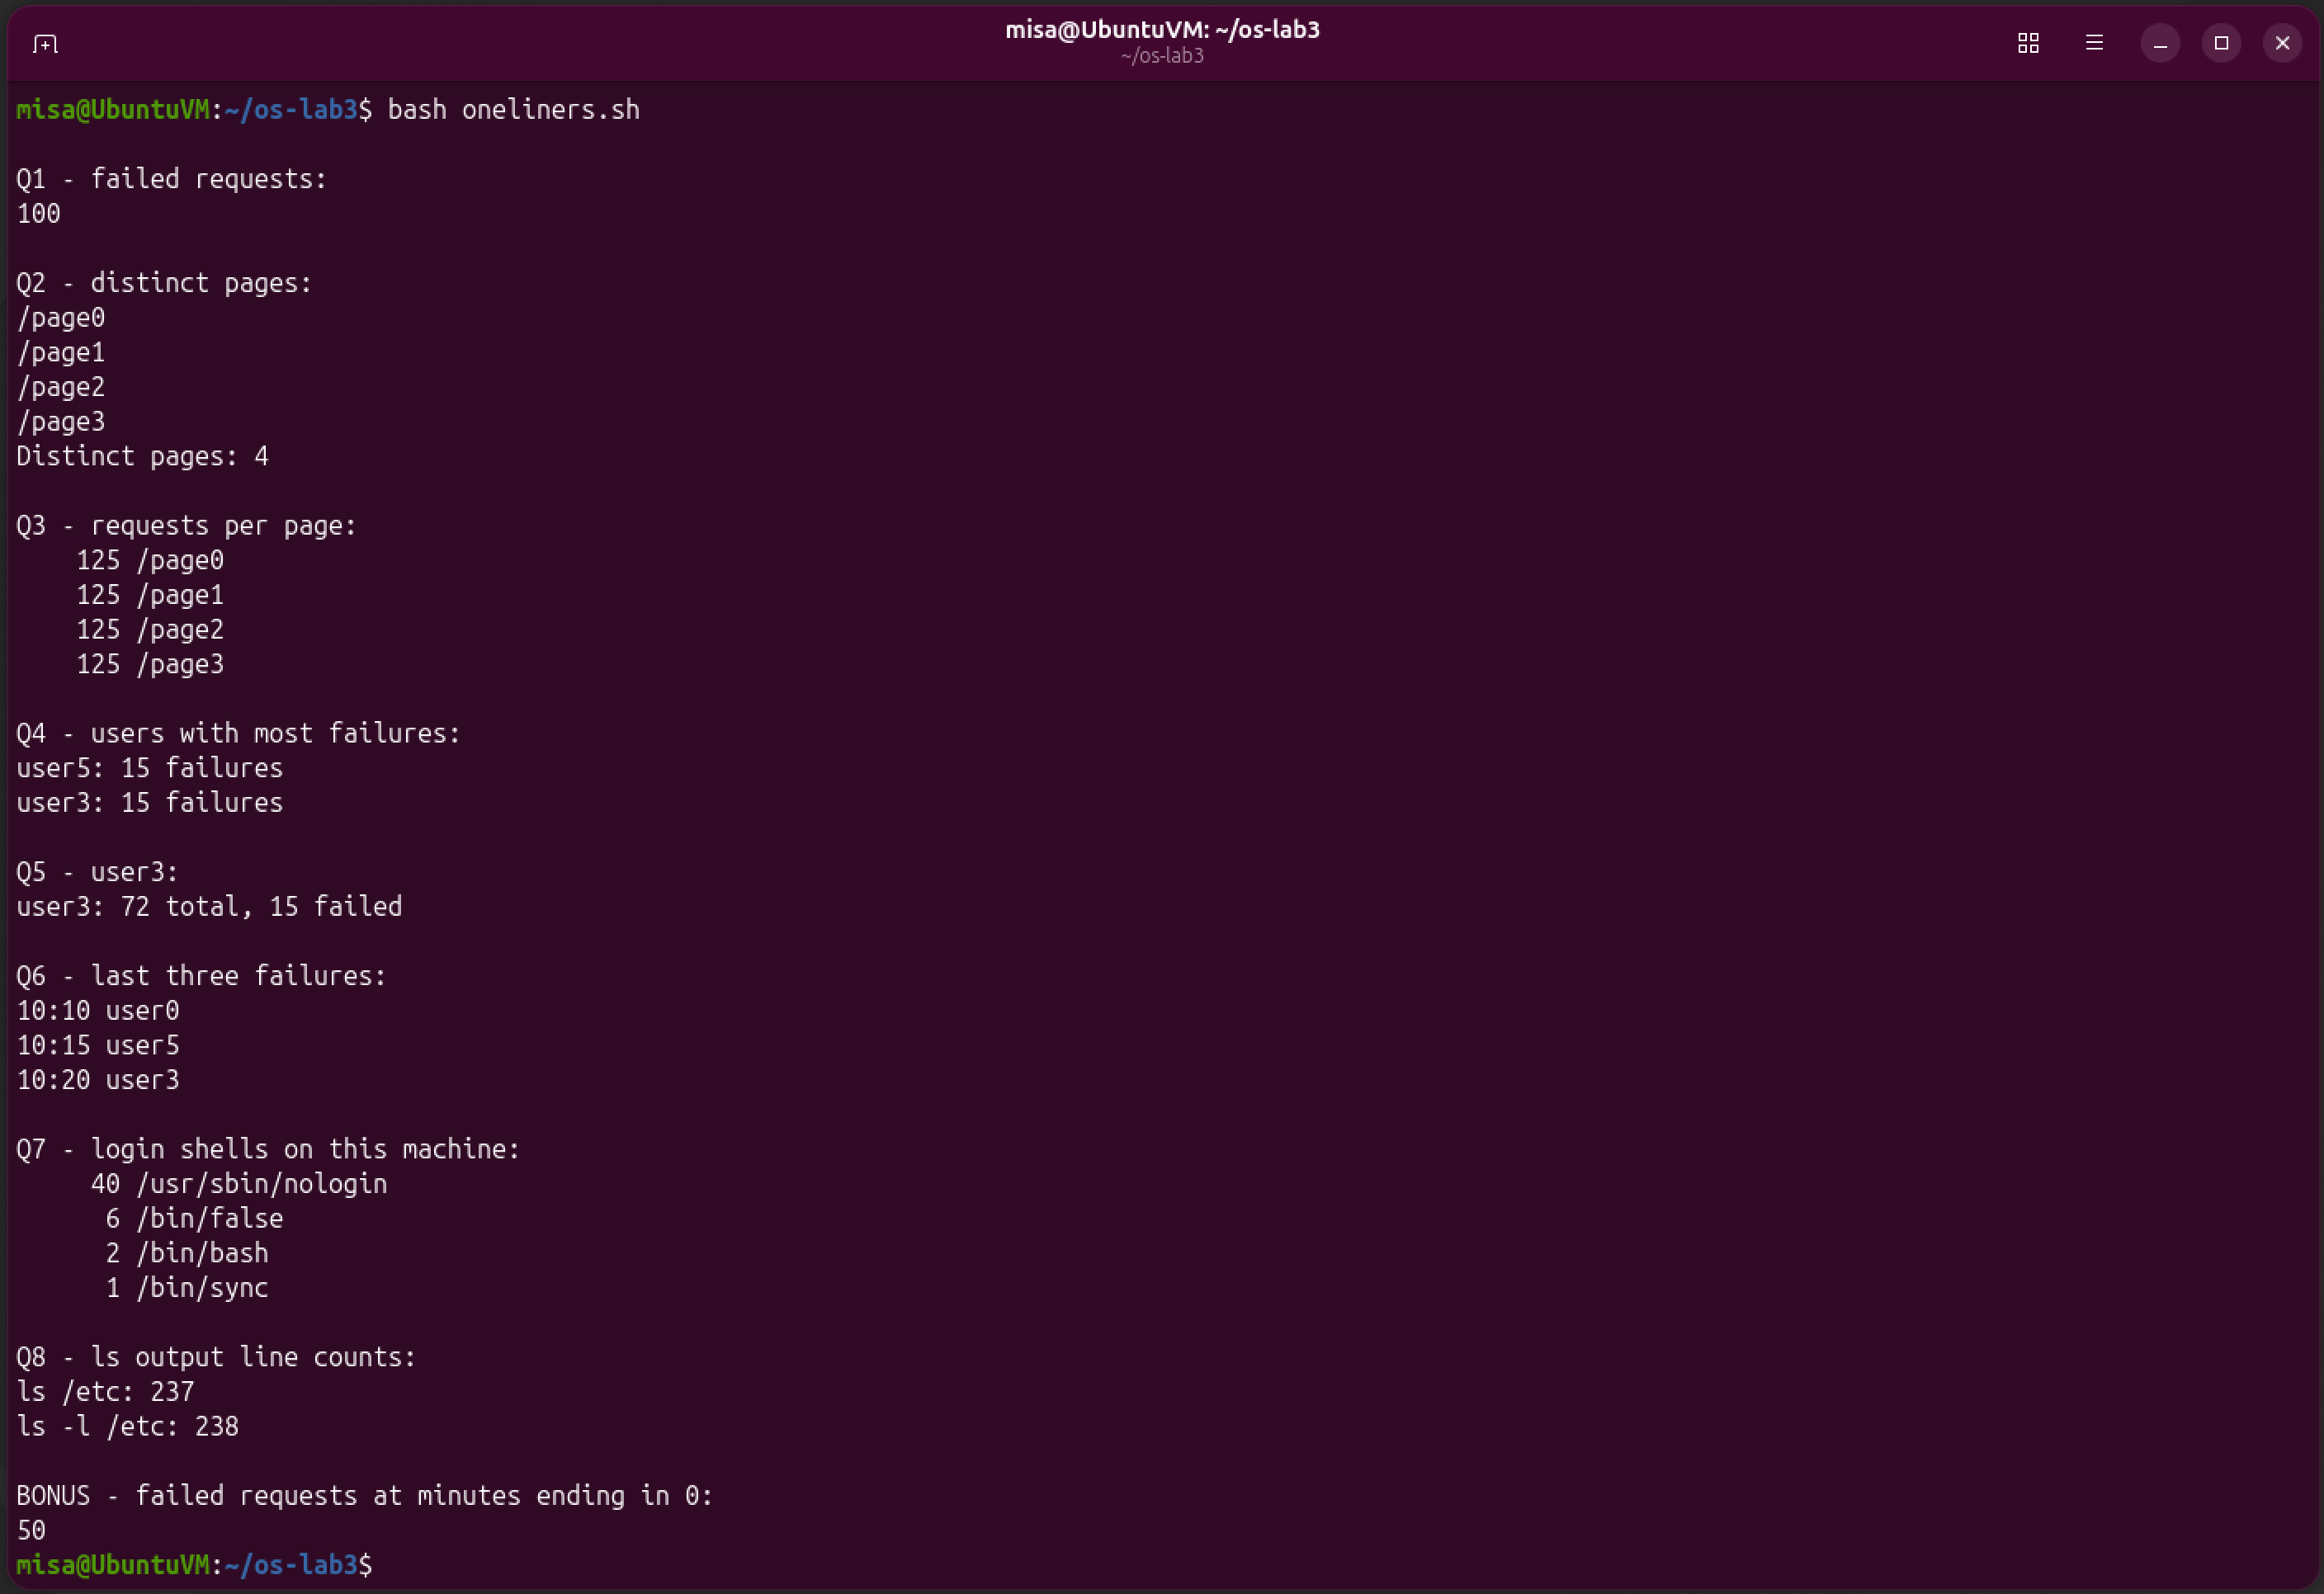
\includegraphics[width=0.88\textwidth,height=0.76\textheight,keepaspectratio]{./img/img_10.png}
    \caption{Results of the oneliners}
    \label{fig:one_liners_log}
\end{figure}


An additional extended regular expression selects failed requests whose
minute ends in zero. The filter matches the six minute values 00, 10, 20,
30, 40, and 50, and produces 50 matching records in the generated log.

\section{My first script}

The most useful filters are collected in \texttt{report.sh}. The script
accepts the path of a log file as its first argument, checks whether the
file exists, and prints the total number of requests and failures.
A loop then counts failures separately for \texttt{user0} through
\texttt{user6}. For the generated log, the totals are 500 requests and
100 failures; each user has 14 failures except \texttt{user3} and
\texttt{user5}, who have 15 each.

The first line, \texttt{\#!/bin/bash}, is the shebang identifying the
interpreter. The executable permission is enabled with \texttt{chmod +x}.
The script is started with \texttt{./report.sh}, since the current
working directory is not among the configured \texttt{PATH} entries.
For a missing log file, the script writes its error to standard error
using \texttt{>\&2} and exits with status 1.

\begin{figure}[H]
    \centering
    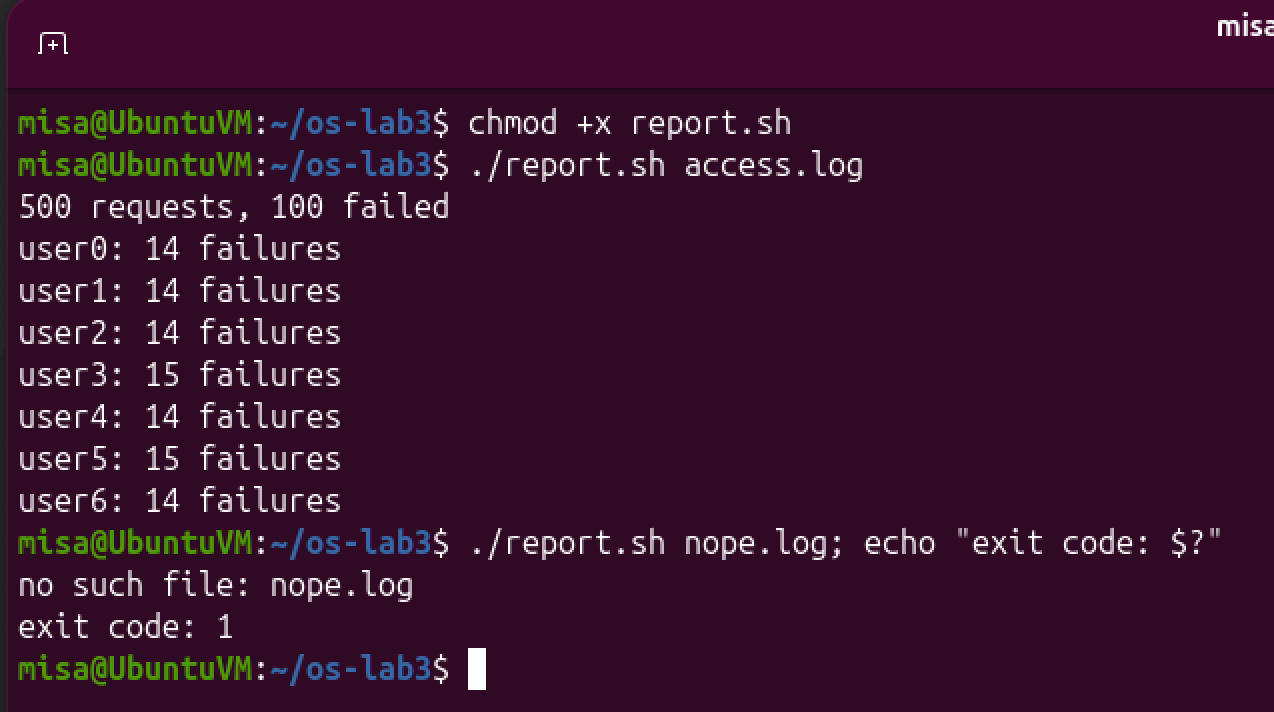
\includegraphics[width=0.88\textwidth,height=0.76\textheight,keepaspectratio]{./img/img_12.png}
    \caption{Running report.sh with a valid and a missing input file}
    \label{fig:report_script}
\end{figure}

For the scheduling exercise, a user crontab entry runs the script once
per minute using absolute paths. Its output is appended to
\texttt{report.log}; \texttt{2>\&1} also captures error messages.
After two scheduled executions, the log is inspected and the added
crontab entry is removed.

\begin{figure}[H]
    \centering
    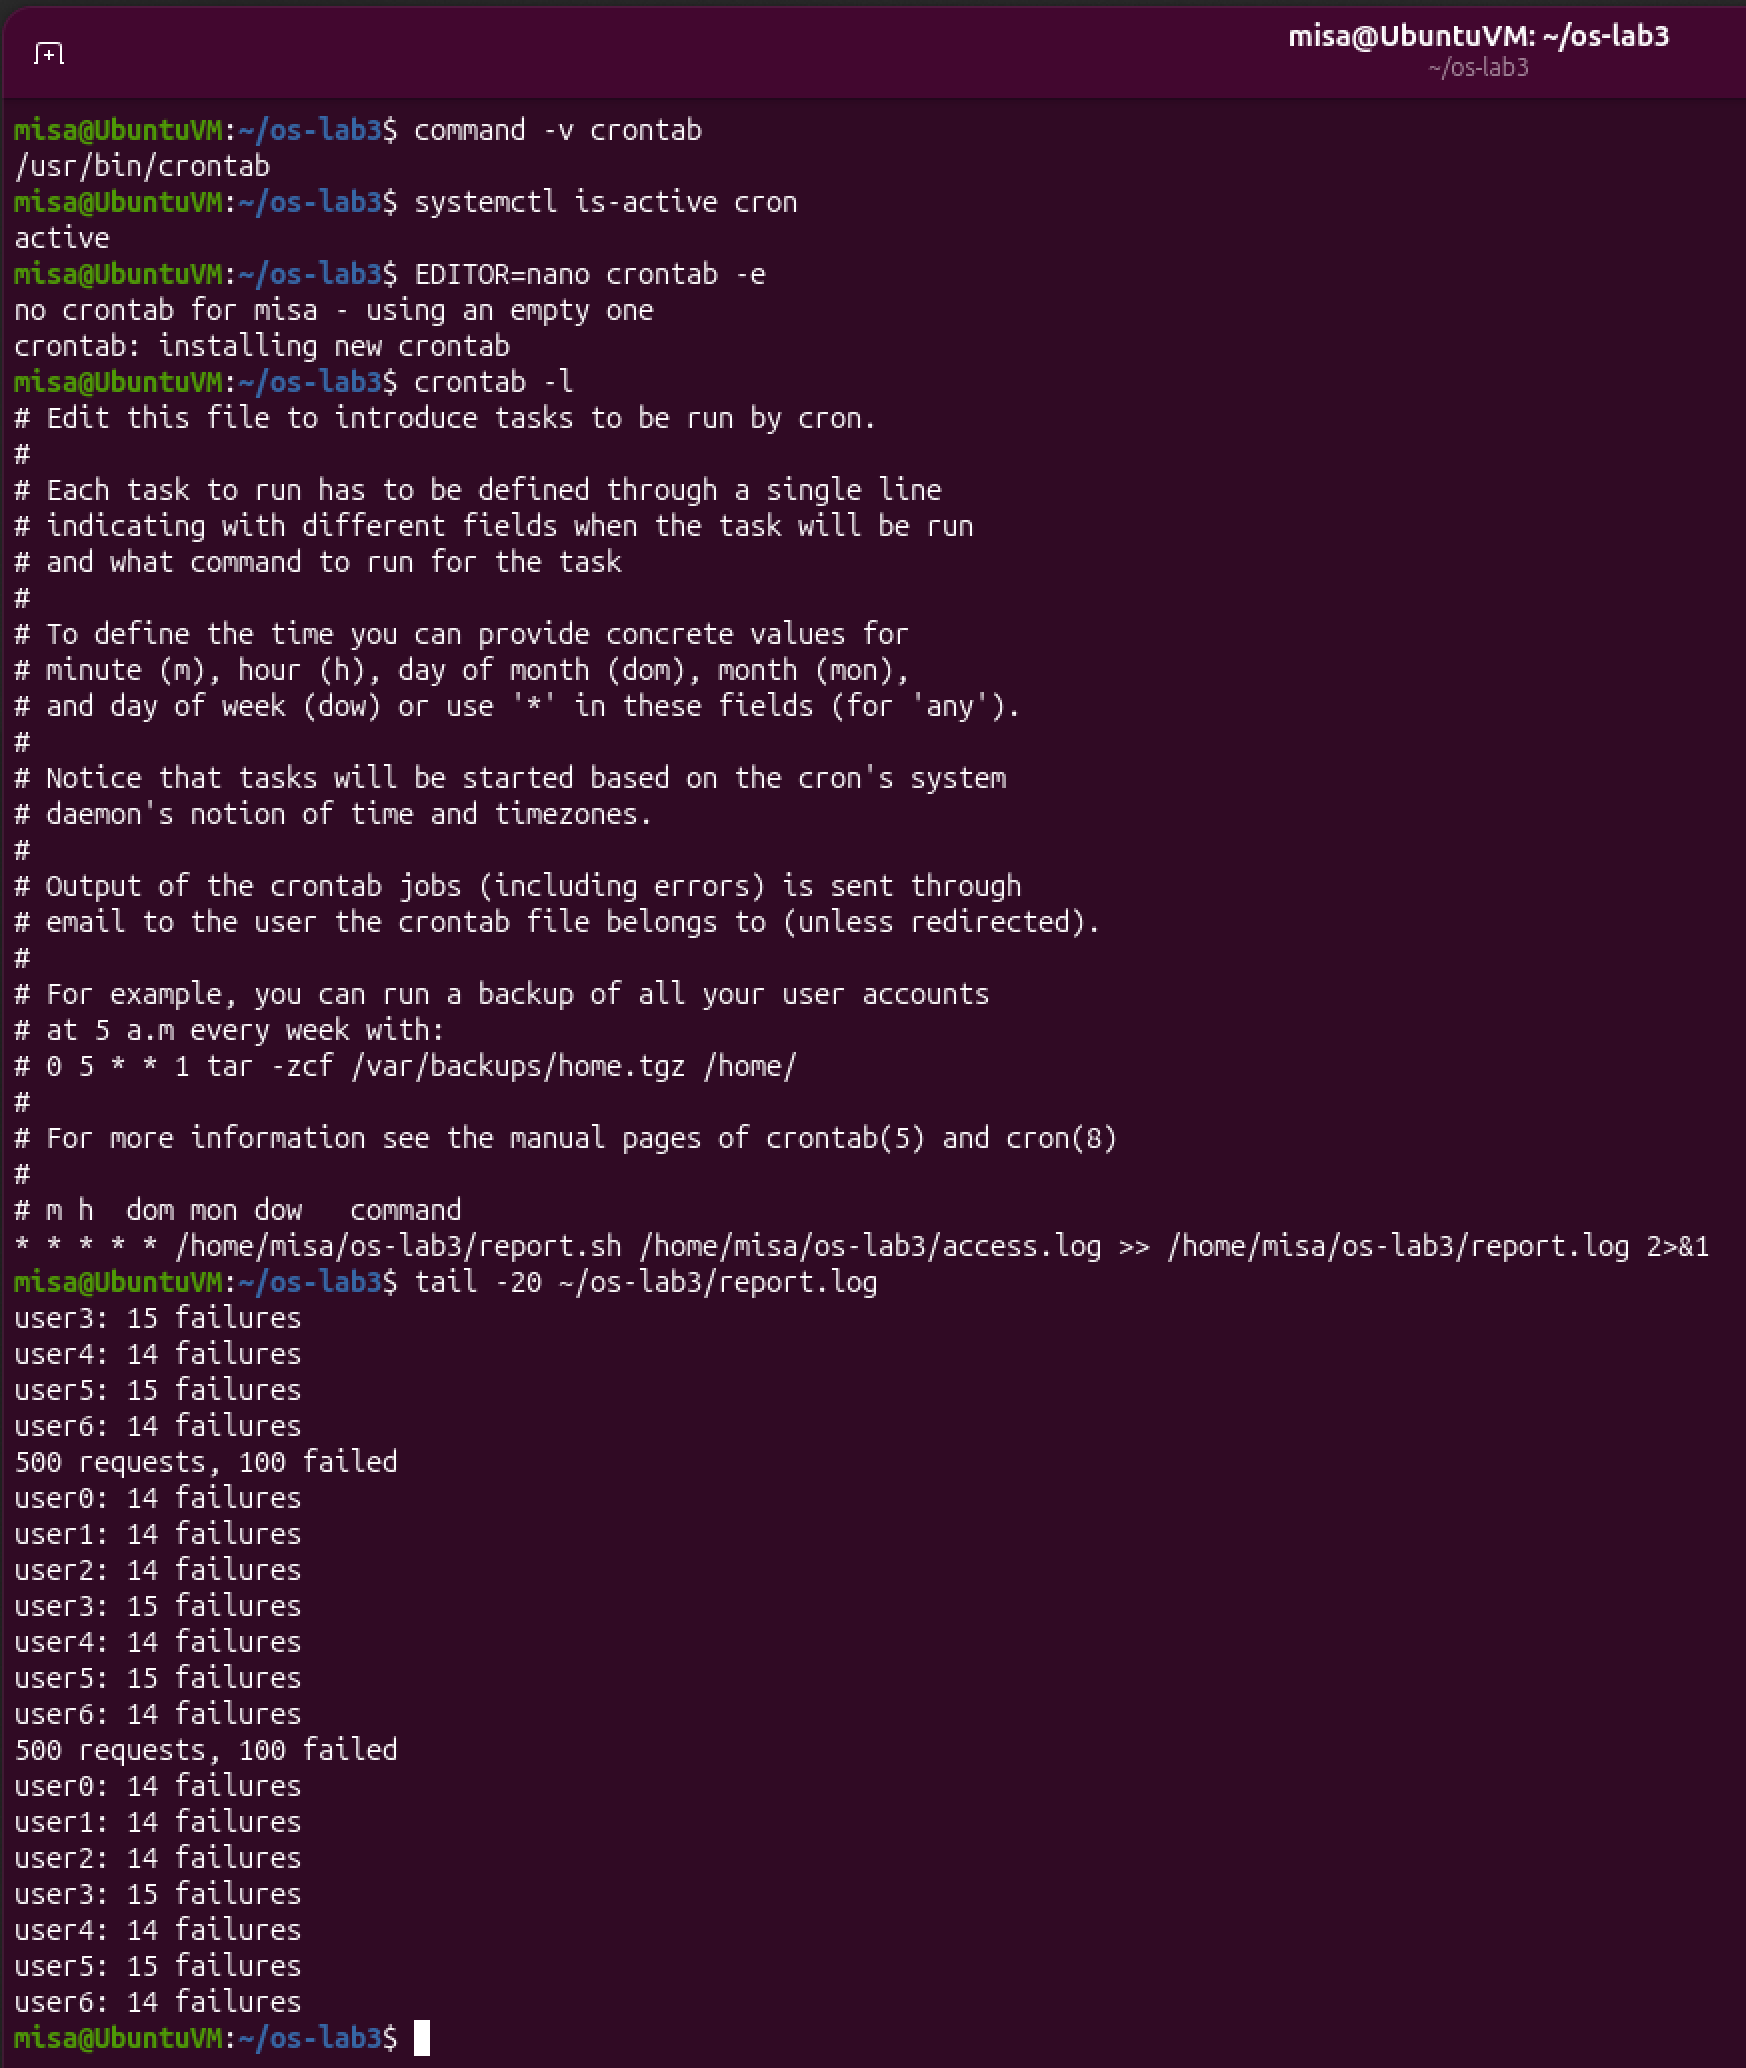
\includegraphics[width=0.88\textwidth,height=0.76\textheight,keepaspectratio]{./img/img_13.png}
    \caption{Cron schedule and successive entries in report.log}
    \label{fig:report_cron}
\end{figure}

\begin{figure}[H]
    \centering
    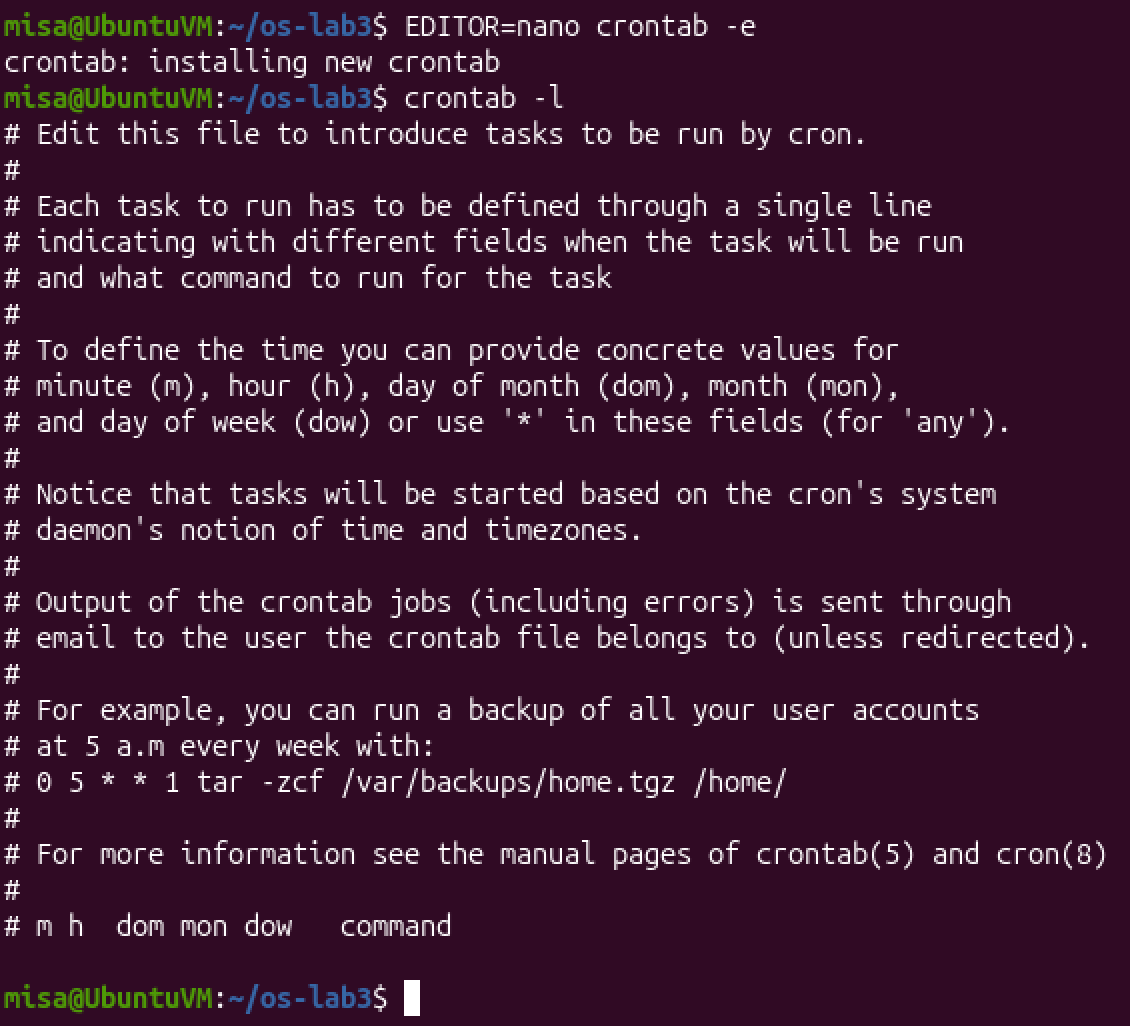
\includegraphics[width=0.88\textwidth,height=0.76\textheight,keepaspectratio]{./img/img_14.png}
    \caption{Verifying removal of the temporary cron entry}
    \label{fig:cron_removed}
\end{figure}

% =======================================================================
\chapter{CONCLUSIONS}
% =======================================================================

The exercises showed how Bash transforms a command line before invoking a
program and how its built-ins, command history, completion, and manual pages
support efficient work in the terminal. Filename expansion, quoting,
variable substitution, redirection, and conditional execution were observed
directly in the shell.

Text filters and pipelines made it possible to extract useful statistics
from a 500-line access log without manually examining each record.
The resulting script combines those operations into a reusable report,
including input validation and per-user failure counts. Scheduling that
script with cron extends the same command-line techniques to recurring
system tasks.

\clearpage
% =======================================================================
% Bibliography
% =======================================================================
% \begin{thebibliography}{99}
\singlespace \normalsize

% \bibitem{ref:Chicago}
%   The Chicago Manual of Style.
%   "Notes and Bibliography: Sample Citations".
%   Accessed October 14, 2022.
%   \url{https://www.chicagomanualofstyle.org/tools_citationguide/citation-guide-2.html}.

% \bibitem{ref:Cats}
%   Google.
%   "Search results for cats".
%   Accessed August 15, 2023.
%   \url{https://www.google.com/search?q=cats}.

\bibitem{ref:OS-GfG}
  GeeksforGeeks.
  "What is an Operating System?".
  Last Updated July 25, 2025.
  Accessed October 16, 2025.
  \url{https://www.geeksforgeeks.org/operating-systems/what-is-an-operating-system/}.

\bibitem{ref:OS-concept}
Silberschatz, A., Galvin, P. B., \& Gagne, G. (2018).
\textit{Operating System Concepts} (10th ed.).
Wiley.
ISBN 978-1-119-32091-3.

\end{thebibliography}


\clearpage
\end{document}
